\newcommand{\mypathoj}{../thesis/oj}

\newcommand{\mypathojdata}{../thesis/oj/data}
\newcommand{\alert}[1]{#1}
\chapter{Reducing~Cascading~Risk~Through  Real-Time~Dispatch}\label{ch:jccow}

Large scale load shedding events caused by cascading power failures have an extreme impact on.  As seen in \cref{intro-chapter}, the costs of these single events can be in the billions, put a halt on commercial and industrial activities, and even cause the loss of life.  Since these events are rare, their can be hard to quantify, and creating useful models to help mitigate this risk is difficult.

\section{OPA and JCC review}
In \cref{msip-model}, we explore the models of power flow over topological networks, cascading risk models, and a system equilibrium model (OPA) in which there is a balance found between economic efficiency and reliability.  For economic reasons, power systems move towards critical points, which are points of maximum throughput for the given infrastructure and are characterized by power flow being limited by either transmission constraints or generation capacity limits.  A critical point primarily due to transmission constraints will lead to larger blackouts, however infrequently, and a critical point primarily due to generation capacity will lead to smaller blackouts that are more frequent.  In the OPA model, there is an engineering response to these blackouts to improve the infrastructure.  An equilibrium is found in the distribution of blackout size such that the load shed for these events follow a power tail distribution.  This equilibrium has been seen in the real world, the distribution of load shed events follow a power tail distribution with exponent $-1.3 \pm .2$ and has stayed the same for 30 years.  We model the short term cascading process as a multi-stage stochastic program that can be embedded in design problems.

In \cref{dfo-chapter}, we decompose the MSIP model by scenario and use a fast monte carlo simulation approach that is parallelizable to evaluate the load shed distribution given demand and contingency scenarios.  Here we aim to improve the system before an event occurs.  As we saw in the Northeast Blackout of 2003, once things go wrong, events that the system is typically robust to can compound and eventually lead to large scale blackout.  For example, after losing the Stuart-Atlanta 345 kV line, the fact that MISO was unaware of this event, led to the inability to provide support in dealing with this problem.  One way to reduce the likelihood of these rare events is to reduce the likelihood of the initiating contingencies.  We proceeded to explore this load shed distribution by looking at the design problem of increasing capacity on transmission elements and the effects it has on the OPA simulation.  This OPA simulation has a natural connection with our risk model that we will explore in this chapter.

In \cref{jcc-chapter}, we developed a model to constrain the probability that one or more lines fail to be small.  This is in line with the idea in \cref{dfo-chapter} where we would like to reduce the likelihood of initiating events occuring.  To start, we noted that due to the increased penetration in renewables and modern technologies of electric vehicles and energy storage, it is vital to include uncertainty of net injections into the model.  We then look at the chance constraint models in literature that deal with this uncertainty in net injections.  Another interesting class of models in literature approached the reliability problem from a system perspective.  Since we don't want any lines to fail, we develop a joint chance constraint on the probability that one or more lines fail.  In order to model this, we assume that the failure density function of an individual line is a piecewise linear function and that line failure probabilities are independent of each other given the branch flow.  However, the branch flow is certainly correlated, as it is the flows on fixed topological structure with fixed power flow parameters.  For the DC approximation of power flows, the branch flows follow a linear relationship with net injections.  If we assume that the net injections are a multivariate Gaussian with a known covariance matrix it follows that the branch flows are multivariate Gaussian and we can calculate its covariance matrix.  We now make our first approximation by taking a linearization ofthesystem risk measure using a Taylor expansion and dropping higher order terms.  This is a very good approximation for small failure probabilities and it allows us to pass this multivariate Gaussian through our piecewise linear failure density function.  We finish this model by calculating the expected probability of a line failing for each branch and then sum over all branches to get our system risk measure, which is constrained.


The downside of a chance constrained model is that it does not account for the impact of failure events.  Power system networks are comprised of many different classes of assets.  The most straightforward example is that the failure of a small distribution line in a radial tree will have minimal impact on the reliability of the bulk power system and the high voltage network that carries the majority of the power over long distances.  However, even among the bulk power system, the failure of individual lines may have disproportionate impact on the probability of a large scale cascading event.  This may have to do with many things such as the connectivity of a neighboring node, the current environmental conditions in and around a region, or even the relay settings on neighboring transmission lines.  Here we will take an empirical approach using the OPA cascading simulation from \cref{dfo-chapter} to evaluate the impact of losing a line on the resulting cascade simulation and the output of the load shed distribution.  We then incorporate this measure of impact into our JCC model by giving it an OPA weighting scheme, denoted JCC-OW (Joint Chance Constraint - OPA Weighted).  This OPA weighting scheme can be thought of as a surrogate model for OPA to be used in a real time dispatch model.  This problem is solved with a cutting plane algorithm similar to JCC.  Finally, we explore the trade-off between cost of dispatch and rare event risk through the computational section.




\section{Cascading Failure Risk Model}
We would like to take into account the impact of losing a transmission element on the load shed distribution from OPA.  Instead of being concerned with only whether or not a line fails, we would also like to know how much does this line contribute to cascading power failure risk.  Due to reliability requirements such as N-1 constraints, the base system is typically stable and has low cascading power failure risk.  Since outages can be due to things outside of system control, we will perform our risk analysis under N-1 exogenous contingencies corresponding to each individual line outage.  After these initial line outages, the system is sometimes moved to a state where additional outages may begin a cascading process leading to a large load shed event.  We will use these N-1 contingencies as well as our JCC risk model to sample initial contingencies for the OPA cascading process.  The initial contingency will include the line that failed with certainty due to an exogenous event as well as probable line outages due to current flow on transmission elements and the given failure density function.  We will use the distribution of load shed after the OPA process to develop an OPA weighting for JCC to take into account the effects of the particular line on the cascading process. 

\subsection{Overview of Sources of Uncertainty}

\begin{figure}
\centering
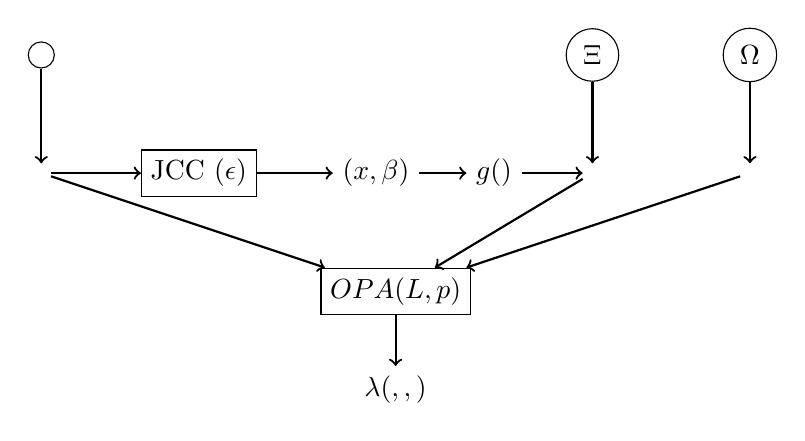
\begin{tikzpicture}

\draw (0,3.5) node(demand)[circle,draw]{ $\bD$};
\draw (7,3.5) node(contingency)[circle,draw]{ $\Xi$};
\draw (9,3.5) node(evolution)[circle,draw]{ $\Omega$};

\draw (0,2) node(rd){ $\rd $};
\draw (2,2) node(JCC)[rectangle,draw]{ JCC $(\epsilon)$ };
\draw (4.25,2) node(rf){ $\ry(x,\beta)$};
\draw (5.75,2) node(grf){ $g(\ry)$};
\draw (7,2) node(rxi){ $\rxi$};
\draw (9,2) node(romega){ $\romega$};
\draw (4.5,.5) node(ropa)[rectangle,draw]{ $OPA(L,p)$};
\draw (4.5,-.75) node(rlambda){ $\lambda(\rd,\rxi,\romega)$};

\draw[thick,->] (demand) -- (rd);
\draw[thick,->] (rd) -- (JCC);
\draw[thick,->] (JCC) -- (rf);
\draw[thick,->] (rf) -- (grf);
\draw[thick,->] (grf) -- (rxi);
\draw[thick,->] (contingency) -- (rxi);
\draw[thick,->] (evolution) -- (romega);
\draw[thick,->] (rd) -- (ropa);
\draw[thick,->] (rxi) -- (ropa);
\draw[thick,->] (romega) -- (ropa);
\draw[thick,->] (ropa) -- (rlambda);

\end{tikzpicture} 
\caption{Random variable relationships and sources of uncertainty}
\end{figure}

We are capturing three separate sources of uncertainty and evaluating the stress on the power system by using the OPA cascading model as a surrogate process for the risk of a cascading power failure.  The power system is affected daily by the uncertainty in demand and generation, denoted by random variable $\rd = d + C_m \ri$ with  probability space $\bD$.  We built this uncertainty into our model and by assuming the net injection uncertainty is multivariate Gaussian, we calculate a system risk measure approximating the probability that one or more lines fail.  This ties into the next source of uncertainty, random variable $\rxi$ for probability space $\Xi$, which models the initial line failures that could initiate a cascading sequence.  This random variable, $\rxi$, will provide the connection between the JCC model of \cref{jcc-chapter} with the OPA model from \cref{msip-model,dfo-chapter}.  The primary source of uncertainty modeled in those chapters was $\romega$ from space $\Omega$ which governs the evolution of the cascading model.  This cascading model can be seen as a surrogate for the stress on the power system in relation to rare event failures.     

The JCC model incorporates uncertainty from random demand, $\bD$.  The outcome of the JCC model is random branch flows, and using the failure density function, we find a distribution of initial contingencies $\Xi$.  The OPA model incorporates uncertainty from all three sources, the demand $\bD$, the initial contingencies $\Xi$, and the cascade evolution $\Omega$.  Let $\cX = \bD \times \Xi \times \Omega$ represent the whole probability space for the OPA model, where $\rchi = (\rd, \rxi, \romega)$ is an event in the whole sample space.  The random variables dependencies are laid out in figure (ref) that describe the relationships between variables.



\subsection{N-1 Exogenous Contingencies}

\begin{figure}
\centering
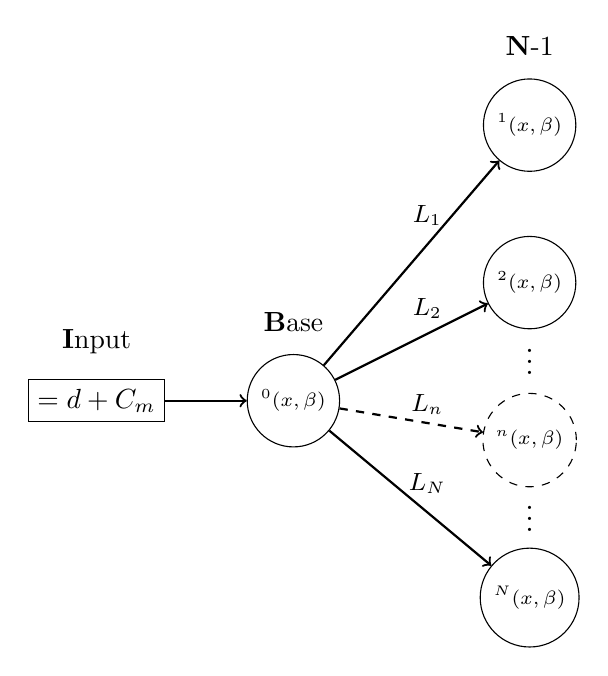
\begin{tikzpicture}

\draw (-2,1.25) node{ \textbf Input };
\draw (-2,.5) node(INPUT)[rectangle,draw]{ $\rd=d + C_m \rdelm$};
\draw (.5,1.5) node{ \textbf Base };
\draw (.5,.5) node(ROOT)[circle,draw]{\scriptsize $\ry^0(x,\beta)$ };
\draw (3.5,5) node{ \textbf N-1 };
\draw (3.5,4) node(ONE)[circle,draw]{ \scriptsize $\ry^1(x,\beta)$ };
\draw (3.5,2) node(TWO)[circle,draw]{ \scriptsize $\ry^2(x,\beta)$ };
\draw (3.5,1.1) node(DOTONE){ \large $\vdots$ };
\draw (3.5,0) node(N)[circle,dashed,draw]{ \scriptsize $\ry^n(x,\beta)$ };
\draw (3.5,-.9) node(DOTTWO){ \large $\vdots$ };
\draw (3.5,-2) node(S)[circle,draw]{ \scriptsize $\ry^N(x,\beta)$ };

\draw (2.2,2.85) node(OMG1){ \small $L_1$ };
\draw (2.2,1.67) node(OMG2){ \small $L_2$ };
\draw (2.2,.45) node(OMG){ \small $L_n$ };
\draw (2.2,-.55) node(OMGS){ \small $L_N$ };


\draw[thick, ->] (INPUT) -- (ROOT) ;
\draw[thick, ->] (ROOT) -- (ONE) ;
\draw[thick,->] (ROOT) -- (TWO);
\draw[thick,dashed, ->] (ROOT) -- (N);
\draw[thick,->] (ROOT) -- (S);

%\draw[thick,dashed] (TWO) -- (N);
%\draw[thick,dashed] (N) -- (S);

\end{tikzpicture} 
\caption{N-1 Exogenous Contingencies}
\end{figure}


Reliability standards in power systems include N-1 contingency constraints.  The system must be robust to failures of each individual component due to reasons outside of the control of the system. The branch flows for line $e$ given contingency $n$ can be described with the following relationship
\begin{equation}\label{n1cont}
 \ry_e^n = \ry_e + L_{e n} \ry_n 
\end{equation}
with $L_{en}$ being a line outage factor for outage $n$'s effect on line $e$.  In \cref{jcc-chapter} we saw the injection shift factor $A$ that gave the change in branch flows depending on changes in net injection.  Here, we will use the branch shift factor $A^B$ where the individual entry $A_{e_1 e_2}^b = \frac{ dy_{e_1}}{dy_{e_2}}$ give the change in branch flow of branch $e_1$ when branch $e_2$ flow is changed and is detailed in \cite{matpower}.  We can calculate the branch shift factor by applying our branch incidence matrix to the injection shift factor in matrix form as 
\begin{equation}
A^B = A C^T.
\end{equation}
 Then the line outage factor can be found by applying a scale factor so that when the line outage factor is multiplied by the branch flow, the response to all other branches is found.  
\begin{equation}\label{line_outage}
L_{en} = \left\{ \begin{array}{c c}
  -1 & \mbox{ if } e=n\\
  A_{en}^B (1-A_{nn}^B)^{-1} & \mbox{ if } A_{nn}^B \neq 1\\
  \mbox{NaN} & \mbox{ o/w }
  \end{array}
\right.
\end{equation}
Shift factors for multiple lines can be found provided certain conditions are met and are explained in \cite{guler_2007}.  However are typically only used for a small number of line outages.  A subset of lines will not have line outage factors when $A_{nn}^B = 1$, and in our computational results, we filter out these scenarios for the N-1 analysis.


The mean flow in contingency $n$ can be found by taking the expectation over the uncertainty in net injections and using \cref{n1cont} that describes flow for branch $e$ in contingency $n$.
\begin{equation}
\E{\bD}{\ry_e^n} =  \E{\bD}{\ry_e}  + L_{en} \E{\bD}{\ry_n} 
\end{equation}
We also need to understand the standard deviation of branch flows in the N-1 contingencies in order to form the JCC constraint for each contingency.  Calculating the variance of $\ry_e^n$ and expanding out using \cref{n1cont}, we see that the variance of branch flow is
\begin{subequations}
\begin{align}
 \operatorname{Var}[\ry_e^n] &= \operatorname{Var}[\ry_e] + L^2_{e n} \operatorname{Var}[ \ry_n ] + 2 L_{e n} \operatorname{CoVar}[ \ry_e, \ry_n ] \\
 &= \pi_e^2 \sD - 2 \pi_e \se + \see \nonumber \\
 &\hspace{30pt} + L_{en}^2 \left[ \pi_n^2 \sD - 2 \pi_n \sn + \snn \right] \nonumber \\
 &\hspace{30pt}+ 2 L_{en} \left[ \pi_{e} \pi_{n} \sD -  \pi_{e} \setwo - \pi_{n} \seone   + \seealone \right]  \\
 &= \left[ \pi_e^2 + 2 L_{en} \pi_e \pi_n + L_{en}^2 \right] \sD \nonumber\\
 &\hspace{30pt} - 2 \left[ \pi_e \se + L_{en} \pi_e \sn + L_{en} \pi_n \se + L_{en}^2 \pi_n \sn \right]  \nonumber \\
&\hspace{30pt} +  \see + 2 L_{en} \sen + L_{en}^2 \snn \\
 &=\psen^2 \sD - 2 \psen \left( \se + L_{en} \sn \right) + \sigma^2_{\psi_{en}}
\end{align}
\end{subequations}
by using equation \ref{covar_branch} for the covariance between two branches and simplifying with shift factor
\begin{equation}
\psen = \pi_e + L_{en} \pi_n
\end{equation}
 which captures the slack distribution response to aggregate demand for branch $e$ in contingency $n$.  It is important to note that variance of line flow $e$ in contingency $n$ depends not only on the variance of the individual line flows but also on the covaraince on branch flows $e$ and $n$.  The injection covariance matrix allows you to pre-compute this new parameter $\sigma^2_{\psen}$ which is used in the branch covariance matrix and cutting plane algorithms.  We again use the set of random generation and demand $\cM$ and sum over every combination of $k_1,k_2 \in \cM$.
\begin{equation}
\sigma^2_{\psi_{en}} = \sko \skt \left(A_{ek_1} + L_{en} A_{nk_2}\right)^2 \sigot
\end{equation}
The following equations are added to the JCC model \cref{jcc_program} to describe the mean branch flows in the contingencies as well as the standard deviation of branch flows.  Each contingency has separate line risk variables $z_{en}$ and the system risk is constrained according to that contingencies specific risk level $\epsilon_n$
\begin{subequations}
\label{jcc_n1_program}
\begin{alignat}{3}
\textbf{JCC N1:= }\min & \displaystyle\sum_j \left[  c_2 \left(x_j^2 + \beta_j^2 \sD \right) + c_1 x_j + c_0 \right] && \label{jcc_n1_obj} \\
&\cref{jcc_cons,jcc_kcl,jcc_limit,jcc_gen1,jcc_gen2,jcc_slack,jcc_pi,jcc_var,jcc_lr,jcc_risk}   && \nonumber\\
&y^+_{en} - y_e - L_{en} y_n  \geq 0 && \forall e,n \in \cE \label{n1meanup}\\
&y^+_{en} + y_e  +  L_{en} y_n  \geq 0 && \forall e,n \in \cE \label{n1meandown}\\
 s_{en}^2 - \psen^2 \sD + 2 &\psen \left( \se + L_{en} \sn \right) \geq \sigma^2_{\psi_{en}} && \forall e,n \in \cE \label{n1stddev}\\
&z_{en} - \rho_e(y^+_{en},s_{en}) \geq 0 && \forall e,n \in \cE \label{n1linerisk}\\
&\sum_e z_{en} \leq \epsilon_n && \forall n \in \cE \label{n1riskconst}
\end{alignat}
\end{subequations}
In \cref{n1meanup,n1meandown}, we enforce variable $y^+_{en}$ to be the absolute value of the power flow in branch $e$ for contingency $n$. The standard deviation of branch flow $e$ in contingency $n$ is described by \cref{n1stddev} and is underestimated by the cutting planes that follow.  Additionally, we have \cref{n1linerisk} which describes the individual line risk for every line in every contingency and \cref{n1riskconst} enforces that the system risk level for each contingency is below the chosen risk level $\epsilon_n$.

Finally, in order to describe the convex, non-analytic risk function for the N-1 contingencies \cref{n1linerisk}, we use the same cutting planes from JCC \cref{line_risk_cuts}.  The cutting planes are calculated at a specific value for slack distribution $\beta$ and the line risk function is underestimated via the gradient.  The cutting planes for the standard deviation of branch flow have changed due to the new covariance calculation taking into account the N-1 contingencies.  These equations are as follows.
\begin{subequations}
\begin{align}
s_{en} \geq \fenb &+ \sum_j \pfenb \left( \beta_j - \hat{\beta_j} \right) \label{sd-cut}\\
\fenb &= \sqrt{ \psen^2 \sD - 2 \psen \left( \se + L_{en} \sn \right) + \sigma^2_{\psi_{en}}} \label{sd-calc}\\
  \pfenb &= \frac{\left(A_{ej} + L_{en}A_{nj}\right) \left( \psen \sD - \left(\se + L_{en} \sn \right) \right)}{\sqrt{\psen^2 \sD - 2 \psen \left(\se  + L_{en}\sn \right) + \sigma^2_{\psi_{en}} }} \label{sd-deriv}
\end{align}
\end{subequations}
These equations are used in the cutting plane algorithm, where  \cref{sd-cut} gives an underestimator for the standard deviation of line $e$ in contingency $n$.  To form that equation, we calculate the standard deviation for a fixed slack distribution $\beta$ in \cref{sd-calc} and also the gradient of the standard deviation evaluated at a fixed $\beta$ in \cref{sd-deriv}.




\subsection{Random Initial Contingencies for OPA}
Ideally, given the random branch flow $\ry_e$, the failure density function $g_e(\ry_e)$ represents the probability that each individual line may fail given flow.  In order to make the connection to OPA, we will use this sample space to seed the random initial contingency for the OPA cascading model.  In order to also capture the effects of events outside of our control, we will perform this analysis under the standard N-1 contingencies.  For each N-1 contingency, we have the probabilities that other lines may fail given by $g_e(y_e^n)$ for branch $e$ in contingency $n$.  This means that our OPA cascading model can be seeded by contingencies with one or more initial line failures, governed by the probability distributions of branch flows and uncertainty space $\Xi$.  

The high level sampling process is depicted in  \cref{high_level_sample}. A brief explanation will be given for the sampling algorithm used to seed the random initial contingencies for the OPA model.  The initial contingencies will depend on the uncertainty in demand $\rd$ as well as the controllable injects and slack distribution $(x,\beta)$ found by a dispatch model.  Using the DC assumption, this will give us random branch flows that are a multivariate Gaussian distribution.  We will sample from this distribution to get a realization of branch flows, $y_e$, that we will transform via our failure density function $g(\cdot)$.  Once we have $g_e(y_e)$, we can sample from our second source of uncertainty, $\Xi$, to get  $\xi_e$, a vector of Bernoulli random variables taking 1 with the probabilities $g_e(y_e)$.  This distribution will seed the OPA simulation and then the sampling of the cascade evolution $\Omega$  will govern how the cascade evolves and can be seen in \cref{dfo-chapter}.

\begin{figure}
\centering
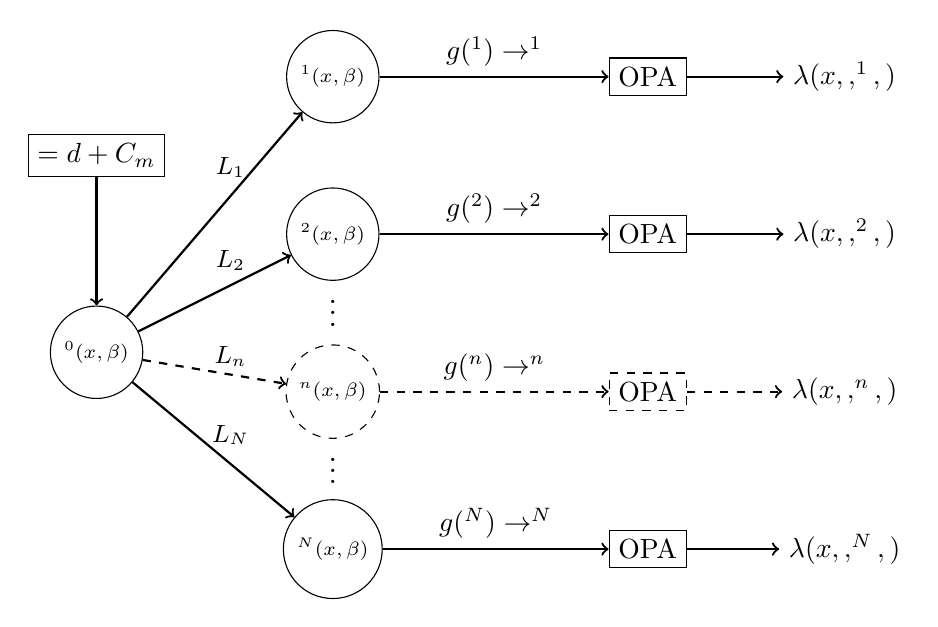
\begin{tikzpicture}

\draw (.5,3) node(INPUT)[rectangle,draw]{ $\rd=d + C_m \ri$};

\draw (.5,.5) node(ROOT)[circle,draw]{\scriptsize $\ry^0(\alert{x},\alert{\beta})$ };
\draw (3.5,4) node(ONE)[circle,draw]{ \scriptsize $\ry^1(\alert{x},\alert{\beta})$ };
\draw (3.5,2) node(TWO)[circle,draw]{ \scriptsize $\ry^2(\alert{x},\alert{\beta})$ };
\draw (3.5,1.1) node(DOTONE){ \large $\vdots$ };
\draw (3.5,0) node(N)[circle,dashed,draw]{ \scriptsize $\ry^n(\alert{x},\alert{\beta})$ };
\draw (3.5,-.9) node(DOTTWO){ \large $\vdots$ };
\draw (3.5,-2) node(S)[circle,draw]{ \scriptsize $\ry^N(\alert{x},\alert{\beta})$ };

\draw (2.2,2.85) node(OMG1){ \small $L_1$ };
\draw (2.2,1.67) node(OMG2){ \small $L_2$ };
\draw (2.2,.45) node(OMG){ \small $L_n$ };
\draw (2.2,-.55) node(OMGS){ \small $L_N$ };

\draw[thick, ->] (INPUT) -- (ROOT) ;
\draw[thick, ->] (ROOT) -- (ONE) ;
\draw[thick,->] (ROOT) -- (TWO);
\draw[thick,dashed, ->] (ROOT) -- (N);
\draw[thick,->] (ROOT) -- (S);

\draw (7.5,4) node(OPAONE)[rectangle,draw]{ OPA  };
\draw (7.5,2) node(OPATWO)[rectangle,draw]{ OPA  };
\draw (7.5,0) node(OPAN)[rectangle,dashed,draw]{ OPA  };
\draw (7.5,-2) node(OPAS)[rectangle,draw]{ OPA };

\draw[thick, ->] (ONE) -- (OPAONE) node [midway,above] { $g(\ry^1) \rightarrow \rxi^1$ };
\draw[thick,->] (TWO) -- (OPATWO) node [midway,above] { $g(\ry^2) \rightarrow \rxi^2$ };
\draw[thick,dashed, ->] (N) -- (OPAN) node [midway,above] { $g(\ry^n) \rightarrow \rxi^n$ };
\draw[thick,->] (S) -- (OPAS) node [midway,above] { $g(\ry^N) \rightarrow \rxi^N$ };


\draw (10,4) node(ONEFIN)[rectangle]{ $\lambda (x,\rd,\rxi^1,\romega )$  };
\draw (10,2) node(TWOFIN)[rectangle]{ $\lambda ( x,\rd,\rxi^2,\romega )$ };
\draw (10,0) node(NFIN)[rectangle,dashed]{ $\lambda ( x,\rd,\rxi^n,\romega )$ };
\draw (10,-2) node(SFIN)[rectangle]{ $\lambda ( x,\rd,\rxi^N,\romega)$ };

\draw[thick, ->] (OPAONE) -- (ONEFIN) ;
\draw[thick,->] (OPATWO) -- (TWOFIN);
\draw[thick,dashed, ->] (OPAN) -- (NFIN);
\draw[thick,->] (OPAS) -- (SFIN);


%\draw[thick,dashed] (TWO) -- (N);
%\draw[thick,dashed] (N) -- (S);

\end{tikzpicture}
\caption{JCC N-1 Risk Model to seed random initial contingencies for OPA}\label{high_level_sample}
\end{figure}




The OPA cascade in this sense is used as a surrogate function to represent rare event risk for a given topology.  The following are the inputs to OPA model that has multiple stages and is solved via multiple LP programs.  The first is the controllable generation $x$, which also indirectly controls the line failure distributions through the intermediate variable $\ry$.  The second input for the OPA model is $\rd$, which is also used directly in our JCC model.  The third input is the initial contingencies $\rxi$, which depends on $\ry$, and thus on $x$ and $\rd$.  Finally, we have $\romega$, which governs the evolution of the cascade process. The load shed for a particular realization of an OPA run is represented by $\lambda$ and is the difference between the nominal load and the load at the last stage of the cascade in the OPA simulation.
\begin{equation}
\lambda ( x, \rd, \rxi, \romega )
\end{equation}
We will be using the expected load shed as a weighting factor to measure the impact of a particular line outage on the OPA cascading process.  For each contingency $n$, we will have a different set of random initial contingencies due to the choice of generation $x$, slack distribution $\beta$ and the resulting random flows $\ry^n$ for each contingency.  The expected load shed for contingency $n$ will be
\begin{equation*}
f_n(x) = \E{\bD, \Xi,\Omega}{ \lambda\left(x,\rd,\rxi^n,\romega\right) }
\end{equation*}



\begin{algorithm}
\caption[Contingency sampling algorithm for OPA]{Contingency Sampling Algorithm for OPA.  Given a dispatch $(x, \beta)$, random demand $\rd=d_0 + C_m \ri$, sample $\rxi^n$ for $T$ trials for each N-1 Contingency \cref{high_level_sample}}\label{opa_sample_alg}
\begin{algorithmic}
\Procedure{SAMPLE}{$x,\beta, \ri, T$}
\State Sample $a=(a_1,a_2,...,a_N)^T$ from independent standard normal distributions.
\State $H H^T = \Sigma^m$ using Cholesky decomposition
\State $\delta^m = H * a$, which will have the desired distribution due to affine transformation
\State $\Delta = \sum_m \delta_m$
\State $x=C_g(x_0 + \beta \Delta)  -(d_0 + C_m \delta^m)$ using \cref{rand_inj} 
\State $y=y_0 + A C_G \beta \Delta - A C_m \delta^m$ using \cref{rand_flow}
\For{$ \forall n \in \cE \mbox{s.t.} A_{nn}^B \neq 1$}
\State $L_{e n} = A^B_{en}(1-A^B_{nn})^{-1}$ using \cref{line_outage}
\State $y_e^n = y_e + L_{e n} y_n$  using \cref{n1cont}
\State $z_e^n = g_e (y_e^n)$

\State $\mathbb{O}^n \gets \emptyset$
\For{$\forall t = 1,2,...,T$}

\For{$\forall e \in \cE $}
\State $\xi_e = 
\left\{ 
\begin{array}{lr}
  1 & \mbox{w/ prob. } z_e^n \\
  0 & \mbox{o/w }
\end{array}
\right. $ 
\EndFor
\State $\mathbb{O}^n \gets \xi$
\EndFor
\EndFor
\State The set $\mathbb{O}^n$ of initial contingencies for each $n$, N-1 contingency, representing distribution $\rxi^n$
\EndProcedure
\end{algorithmic}
\end{algorithm}





\subsection{OPA Weighting for JCC}


While it is important that no lines fail, it may be overly restrictive while not actually reducing the risk of large load shedding events, which is a main concern from a system reliability perspective. It would certainly be more beneficial to keep the large high voltage lines in operation that are critical to system stability versus a few small distribution feeders, which may cause some small load shedding but would keep the bad events contained.  To highlight the downside of chance constrained programming of not capturing the impact of the events, only the probability that they occur, a scatter plot \cref{jcc_and_opa} of the system risk measure of the JCC model and the expected load shed of the OPA model seeded by the random initial contingencies from \cref{opa_sample_alg}, we see there is not a good correlation.  We want to develop a system constraint that is correlated with the expected load shed from the cascading process.

\begin{figure}
\centering
\begin{tikzpicture}[scale=.9]
\begin{axis}[title=Risk Measure vs Load Shed, xlabel=Load Shed, ylabel={$P \left[ \mbox{At least one line fails} \right]$},legend pos=outer north east]
%,ymax=.04%,xmin=\xmmm,xmax=1,
%	  extra x ticks={.8,.9,.98},
%	  extra x tick style={grid=major},
%	  extra x tick labels={}]


  \addplot+[blue,opacity=.85,only marks, mark size=.35] table[x=LS,y=r] {\mypathojdata/jccS1.out};
  \addlegendentryexpanded{JCC}
  \addplot+[blue,opacity=.85,only marks, mark size=.35] table[x=LS,y=r] {\mypathojdata/jccS2.out};
  \addplot+[blue,opacity=.85,only marks, mark size=.35] table[x=LS,y=r] {\mypathojdata/jccS3.out};
  \addplot+[blue,opacity=.85,only marks, mark size=.35] table[x=LS,y=r] {\mypathojdata/jccS4.out};
  \addplot+[blue,opacity=.85,only marks, mark size=.35] table[x=LS,y=r] {\mypathojdata/jccS5.out};


\end{axis}
\end{tikzpicture}
\caption{Line failure risk and OPA not correlated}\label{jcc_and_opa}
\end{figure}


Want a first order weighting, $\eta$, for line risks $z$, to approximate OPA
\begin{align} \label{jcc_ow_weights}
\sum_e \eta_e \E{\bD}{g(\ry_e^n(\alert{x},\alert{\beta}))} &\approx \E{\bD \Xi^n \Omega}{\lambda ( \alert{x},\rd,\rxi^n,\romega) } \\
\eta^T z^n &\approx f_n(\alert{x})
\end{align}


\bc{\begin{figure}
\centering
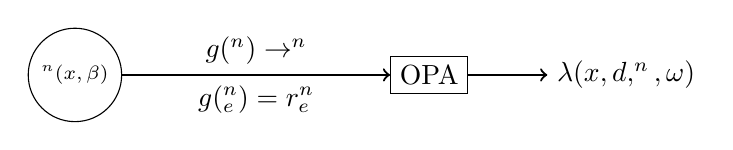
\begin{tikzpicture}
\draw (3.5,4) node(ONE)[circle,draw]{ \scriptsize $\ry^n(\alert{x},\alert{\beta})$ };

\draw (8,4) node(OPAONE)[rectangle,draw]{ OPA  };

\draw[thick, ->] (ONE) -- (OPAONE) node [midway,above] {$g(\ry^n) \rightarrow \rxi^n$ } node[midway,below]{$\E{\bD}{g(\ry_e^n)} = r_e^n$};

\draw (10.5,4) node(ONEFIN)[rectangle]{ $\lambda (\alert{x},d,\rxi^n,\omega )$  };

\draw[thick, ->] (OPAONE) -- (ONEFIN) ;

%\draw<2->[thick,dashed,red] (4.45,3.8) -- (7.2,3.8) -- (7.2,4.8) -- (4.45,4.8) -- (4.45,3.8);
\end{tikzpicture}
\caption{Random initial contingencies and expected failure probabilities}
\end{figure}
}

There are many ways to find a weighting scheme to represent the impact from losing particular lines.  Here is one example that attempts to capture the impact of losing a line with respect to the effect on the expected load shed of the resulting OPA simulations.  For each contingency, a vector of risks, $z^n$, were recorded, which represent the expected probability of that line failing.  For contingency $n$, the probability of line $n$ failing is  $z^n_n=1.$  After performing the OPA simulations, we record the expected load shed $f_n(x)$ for that set of initial contingencies $\rxi^n$.  We formulate the following linear system \cref{solve_opa_weight} and solve for $\eta$.
\begin{equation*}\label{solve_opa_weight}
\begin{bmatrix}  \alert{z^1_1} & \cdots & \alert{z^1_N} \\ \vdots & \vdots & \vdots \\ \alert{z^N_1} & \cdots & \alert{z^N_N} \end{bmatrix}
\begin{bmatrix} \alert{\eta_1}  \\ \vdots  \\ \alert{\eta_N}  \end{bmatrix} 
=
\begin{bmatrix} \alert{f_1(x)}  \\ \vdots  \\ \alert{f_N(x)}  \end{bmatrix} 
\end{equation*}

After applying these new linear weights $\eta$ to the line risks $z$, we find that our new system constraint $\sum_e \eta_e z_e$ is now well correlated with the resulting expected value of load shed of the cascading process as shown in \cref{jcc_ow_correlated}.
In order to solve problems using this weighting scheme, it is nearly identical to JCC N-1 model\cref{jcc_n1_program}, except with the system risk constraint \cref{n1linerisk} representing probability of one or more line failures with the new risk constraint representing the expected value of load shed \cref{jcc_ow_weights}.

\begin{subequations}
\label{jcc_n1_ow_program}
\begin{alignat}{3}
\textbf{JCC N-1 OW:= }\min_{\left(x,\beta,;\theta,y,\pi,s,z\right)} & \displaystyle\sum_j \left[  c_2 \left(x_j^2 + \beta_j^2 \sD \right) + c_1 x_j + c_0 \right] &&  \label{ow_obj}  \\
&\cref{jcc_cons,jcc_kcl,jcc_limit,jcc_gen1,jcc_gen2,jcc_slack,jcc_pi,jcc_var,jcc_lr,jcc_risk}   && \nonumber\\
&\cref{n1meanup,n1meandown,n1stddev,n1linerisk}   && \nonumber\\
&\sum_e \eta_e z_{en} \leq \zeta_n && \forall n \in \cE
\end{alignat}
\end{subequations}

\begin{figure}
\centering
\begin{tikzpicture}[scale=1]
\begin{axis}[title=Risk Measure vs Load Shed, xlabel=Load Shed, ylabel=JCC-OW Risk Measure,legend pos=outer north east]
%,ymax=.04%,xmin=\xmmm,xmax=1,
%	  extra x ticks={.8,.9,.98},
%	  extra x tick style={grid=major},
%	  extra x tick labels={}]


  \addplot+[blue,opacity=.85,only marks, mark size=.35] table[x=LS,y=rl] {\mypathojdata/jccS1.out};
  \addlegendentryexpanded{JCC}
  \addplot+[blue,opacity=.85,only marks, mark size=.35] table[x=LS,y=rl] {\mypathojdata/jccS2.out};

  \addplot+[blue,opacity=.85,only marks, mark size=.35] table[x=LS,y=rl] {\mypathojdata/jccS3.out};

  \addplot+[blue,opacity=.85,only marks, mark size=.35] table[x=LS,y=rl] {\mypathojdata/jccS4.out};

  \addplot+[blue,opacity=.85,only marks, mark size=.35] table[x=LS,y=rl] {\mypathojdata/jccS5.out};


\end{axis}
\end{tikzpicture}
\caption{JCC N-1 OW correlated with OPA} \label{jcc_ow_correlated}
\end{figure}





\subsection{Cutting Plane Algorithm for JCC N-1 with OPA Weighting}
Now, we will describe the algorithm used to solve  JCC N-1 \cref{jcc_n1_program} and the new JCC OW \cref{jcc_n1_ow_program}.  The algorithm for JCC OW will be shown explicitly in \cref{jcc_ow_alg} and the JCC N-1 is nearly identical except for the difference in system risk constraints.
\begin{algorithm}
\caption[Cutting plane algorithm for solving JCC N-1 with OPA weighting]{This cutting plane algorithm solves JCC \cref{jcc_program} with N-1 contingencies\cref{jcc_n1_program} using the OPA weighting scheme \cref{jcc_ow_weights} via linear programs and cutting planes}\label{jcc_ow_alg}
\begin{algorithmic}
\Procedure{JCC N-1 OW}{d,$\Sigma^m$,$\zeta$,$\zeta_n$,L,p}
\State $L \gets \emptyset$  (Set of Lines with potential risk)
\State $S \gets \emptyset$  (Set of Cuts)
\State $r \gets 0$ (Risk)
\BState \emph{solve}:
\State $(\hat{x},\hat{\beta},\hat{y}) \gets $Solve DC Power Flow, \cref{jcc_obj,jcc_cons,jcc_kcl,jcc_slack,jcc_limit,jcc_gen1,jcc_gen2}, with cuts $S$, risk $r\leq\epsilon$
\If {Infeasible} \Return Problem Infeasible 
\EndIf
\State Calculate $\hat{s},\hat{z},\hat{r}$ using $(\hat{x},\hat{\beta},\hat{y})$ and \cref{branch_cov,line_risk}
\If {$\hat{r} \leq \epsilon + tol$} \Return Optimal $(\hat{x},\hat{\beta},\hat{y},\hat{s},\hat{z},\hat{r})$
\EndIf
\For{$\forall e$}
\If {$\hat{z_e} \geq tol$}
    \If {$e \notin L$}
            \State $L \gets \left\{L,e\right\}$
            \State Initialize $s_e,z_e$
            \State $r \gets r + z_e$
    \EndIf            
    \State $S \gets$ line risk cuts \cref{line_risk_cuts} for $z_e,y_e,s_e$ dependent on $\hat{z}_e,\hat{y}_e,\hat{s}_e$
    \State $S \gets$ branch variance cuts \cref{branch_var_cuts} for $s_e,\beta_e$ dependent on $\hat{s}_e,\hat{\beta}_e$
\EndIf
\EndFor
\State \textbf{goto} \emph{solve}
\EndProcedure
\end{algorithmic}
\end{algorithm}



\section{Computational Experiments}
This computational section will just briefly show an example of using the OPA weighting on top of the JCC N-1 risk model. We began by  running JCC N-1 and used it to initiate the N-1 OPA sampling process and ran OPA on each initial contingency.  We created an OPA weighting vector by solving \cref{solve_opa_weight}.  Then we solved JCC OW \cref{jcc_n1_ow_program} using cutting plane algorithm \cref{jcc_ow_alg}.  Finally, we ran the N-1 OPA process again with the two models to determine load shed distribution associated with the two dispatch points.   The goal for JCC OW is to modify the distribution of load shed and reduce the risk of rare event failures that are large.  

To highlight the differences of the JCC OW model, this trial gave a higher budget to the JCC OW model and constrained new system risk measure such that the cost of dispatch was 4\% higher than the standard JCC model.  In return, it was able to reduce the expected value of load shed by 4.7\%, and reduce the 99 percentile of load shed by 28.5\%.  Some statistical measures of the load shed distribution are tabulated in \cref{rare_event_risk_metrics} and plotted in \cref{load_shed_dist_ow}.

\begin{figure}
\centering
\includegraphics[scale=.4]{\mypathoj/histogram-newdes3}
\includegraphics[scale=.4]{\mypathoj/logplot-newdes3}
\caption{Load shed distribution}
\label{load_shed_dist_ow}
\end{figure}


\begin{table}
\centering
Trials \textbf{450400}

\begin{tabular}{|c |  c c | c|}
\hline
Stat & JCC & JCC-OW & diff (\%) \\
\hline
cost&1.78e6 & 1.85e6 & \alert{-3.9} \\
mean&44.0&41.9 & 4.8   \\
num0&199444 & 201984 & 1.3 \\
P95& 138.81& 138.81  &  0         \\
P99& 205.77& 147.12456 &  28.5        \\
P99.8& 441.21& 251.76   &  43      \\
max& 734.29& 612.9      &  16.5            \\
CVaR95 & 182.5 & 155.6 & 14.7 \\
\hline
\end{tabular}
\caption{Rare event risk metrics}\label{rare_event_risk_metrics}
\end{table}


\section{Conclusion}
We extended the JCC model in order to take into account the approximate impact of losing subsets of lines on the resulting OPA cascading process.  We are using the OPA cascading process as an empirical model to represent how stressed the grid is with respect to rare event failures.  The OPA process gives us a distribution of load sheds.  The JCC OW model, which incorporates this linear weighting scheme, was able to change the distribution (for an increased cost) of the resulting load shed by reducing the mean and, even more so, reducing the tail events with large load shed.
